\section{Experimental Results}

The testing adversary and the four criteria we will analyse with our experiments are described in Sec.~(\ref{sec:adversary_description}). \\
For our experiences we consider four scenarios: in each one three of the four parameters $\numTraces[], \numTraces[]', \newTraceLength, \numPoI$ are fixed and one varies. For those in which $\numTraces[]'$ is fixed, the value of $\numTraces[]'$ is chosen high enough to avoid the SSS problem; then, the extensions of LDA presented in Sec.~(\ref{sec:SSS}) are not evaluated.

\subsection{Scenario 1}
\begin{figure}
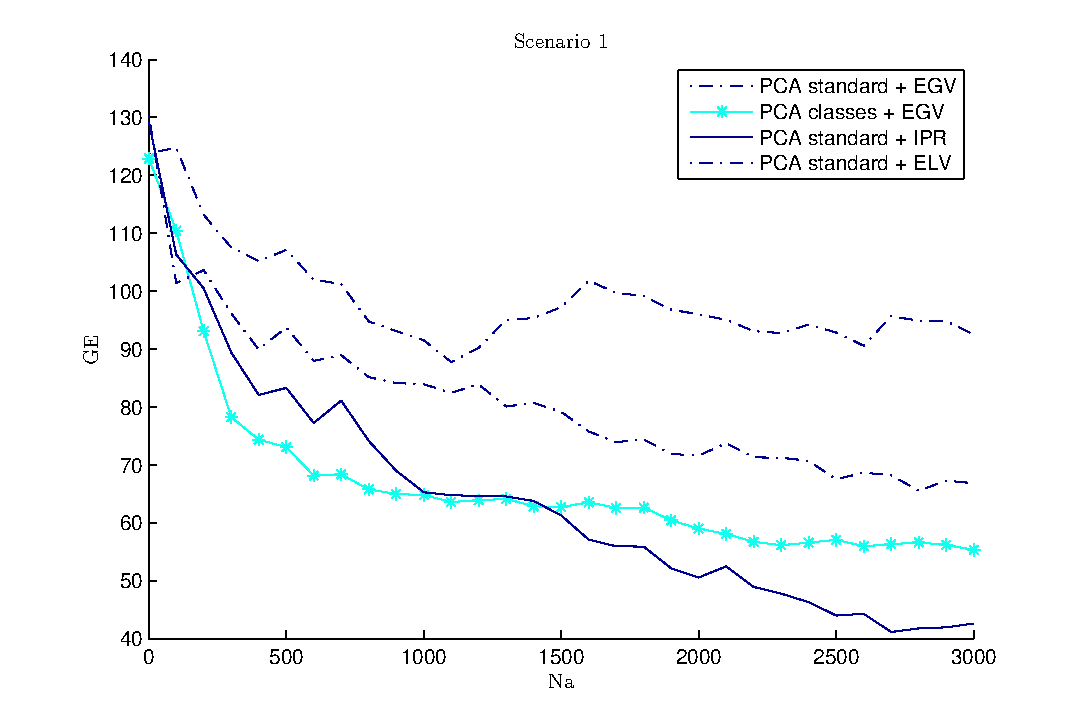
\includegraphics[width=0.5\textwidth]{figures/Criterion1.pdf}
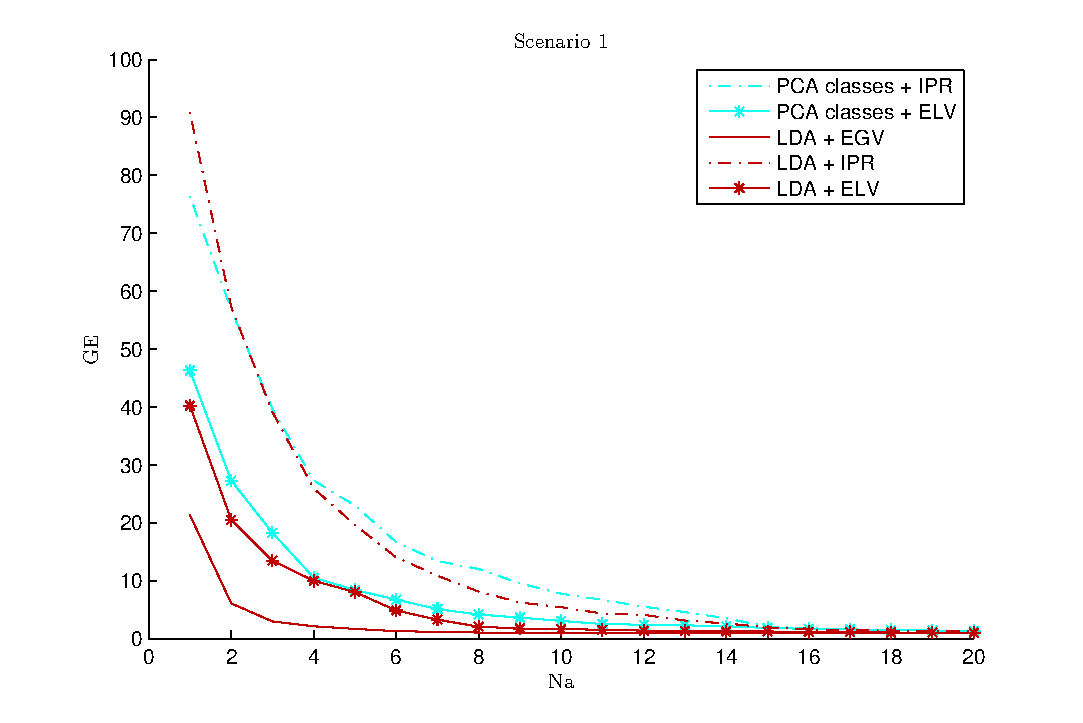
\includegraphics[width=0.5\textwidth]{figures/Criterion1Good.pdf} 
\caption{Guessing Entropy as function of the number of attack traces, for different extraction methods}\label{fig:1}
\end{figure}
To analyse the dependence of our extraction methods on the number of attack traces $\numTraces[]$, we fixed the other parameters as follows: $N_p=50$ ($\numTraces[]'=50*256$), $\newTraceLength = 3$ and $\numPoI = 3996$ (all points are allowed to participate in the building of PCs and LDCs). The experimental results, depicted in Fig.\ref{fig:1}, show that the PCA standard method has very bad performances in SCA, while the LDA is the method that performs best. Concerning the class-oriented PCA, we observe that its performance can be comparable to that of LDA, on condition to be associated to a proper component selection method, ELV (which performs best) of IPR.  \\


\subsection{Scenario 2}
\begin{figure}
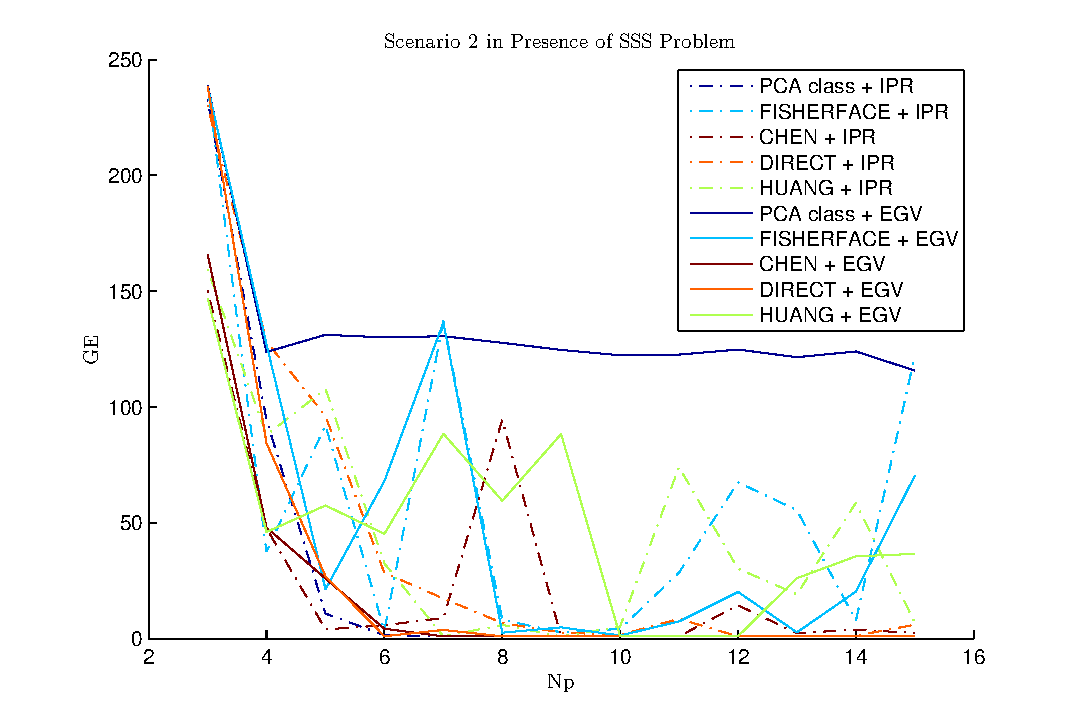
\includegraphics[width=0.5\textwidth]{figures/Criterion2SSS.pdf}
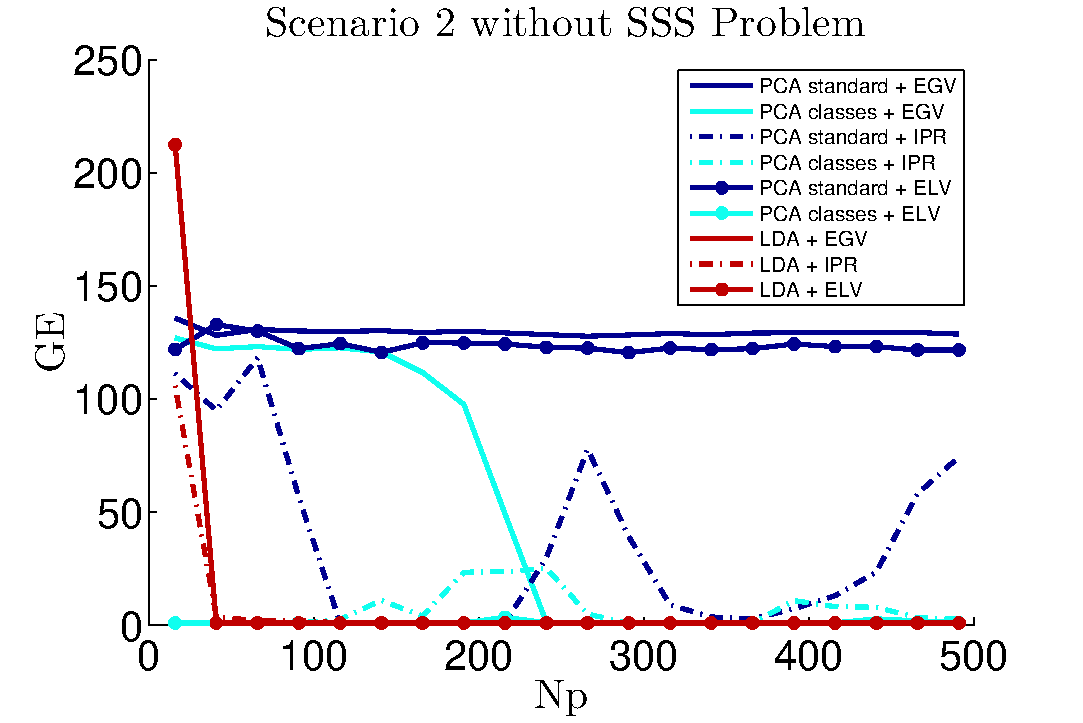
\includegraphics[width=0.5\textwidth]{figures/Criterion2notSSS.pdf} 
\caption{Guessing Entropy as function of the number of profiling traces per class, for different extraction methods: on the left the LDA is substituted by its extensions to handle the SSS problem.}\label{fig:2}
\end{figure}
Now we test the behaviour of the extraction methods, as function of the number $N_p$ of profiling traces per class available. The number of components $\newTraceLength$ is still fixed to 3, and $\numPoI=3996$ again. This scenario has to be divided into two parts: if $N_p\leq 15$, then $\numTraces[]'<\traceLength$ and the SSS problem occurs. Thus, in this case we will test the four extensions of LDA, associated to the standard selection, to which we refer, by abuse, as EGV, that consists in keeping the first $\newTraceLength$ LDCs (except for the Direct LDA, which asks to keep the last LDCs), and to the IPR selection.  We compare them to the class-oriented PCA associated to the same selection methods. The ELV selection is not performed in this case because, for some of the techniques extending LDA, the projecting LDCs are not associated to some eigenvalues in a meaningful way. On the contrary, if $N_p\geq 16$ there is no need to approximate LDA technique, so the classical one is performed. Results for this scenario are shown in Fig.\ref{fig:2}. It may be noticed that the combination class-oriented PCA + IPR does not suffer the lack of profiling traces; anyway, it is outperformed by the Chen method in association to EGV. The Direct LDA method also provide a good alternative, while the other tested methods do not show a stable behaviour. The results in absence of the SSS problem confirm that the standard PCA is not adapted to SCA, even when provided of more profiling traces, and that among class-oriented PCA and LDA, LDA converges faster.



\subsection{Scenario 3}
\begin{figure}
\centering
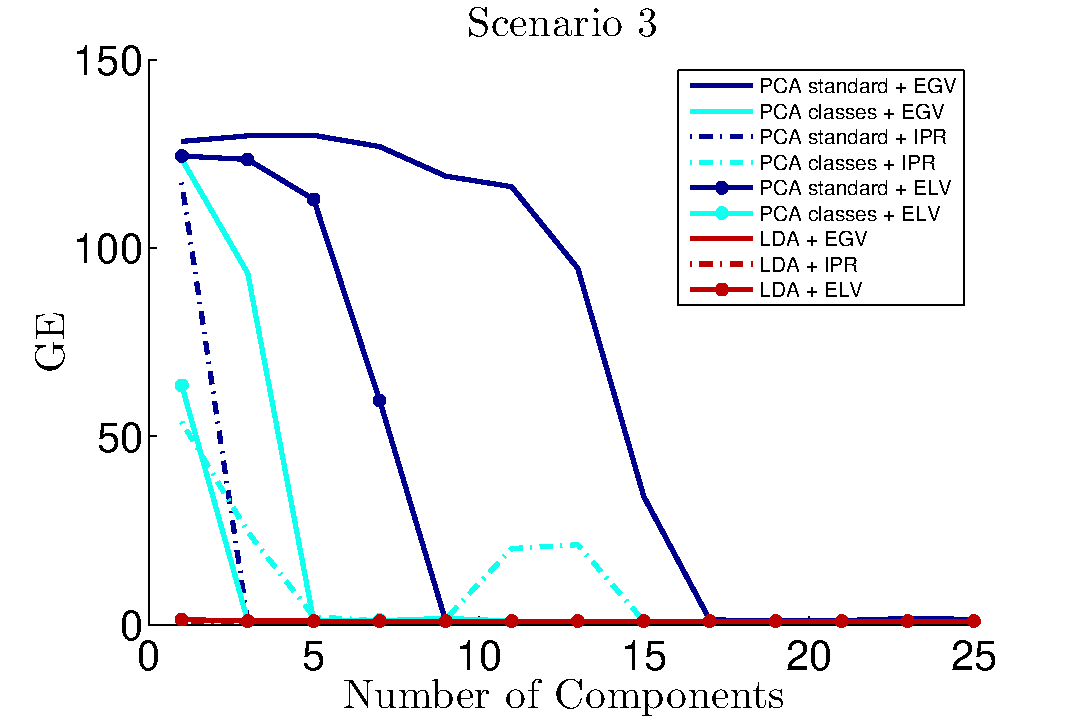
\includegraphics[width=0.5\textwidth]{figures/Criterion3.pdf}
\caption{Guessing Entropy as function of the number of the traces size after reduction.}\label{fig:3}
\end{figure}


Let now $\newTraceLength$ be variable. Other parameters are fixed as follows: $\numTraces[] = 100, N_p=200, \numPoI = 3996$. Looking at Fig.\ref{fig:3}, we might notice that what standard PCA asks to well perform in SCA context, is a larger number of kept components; on the contrary, a little number of components suffices to the LDA. Finally, keeping more of the necessary do not worsen the efficiency of the attack, which allows adversary to choose $\newTraceLength$ as the maximum value supported by their computational means.



\subsection{Scenario 4}
\begin{figure}
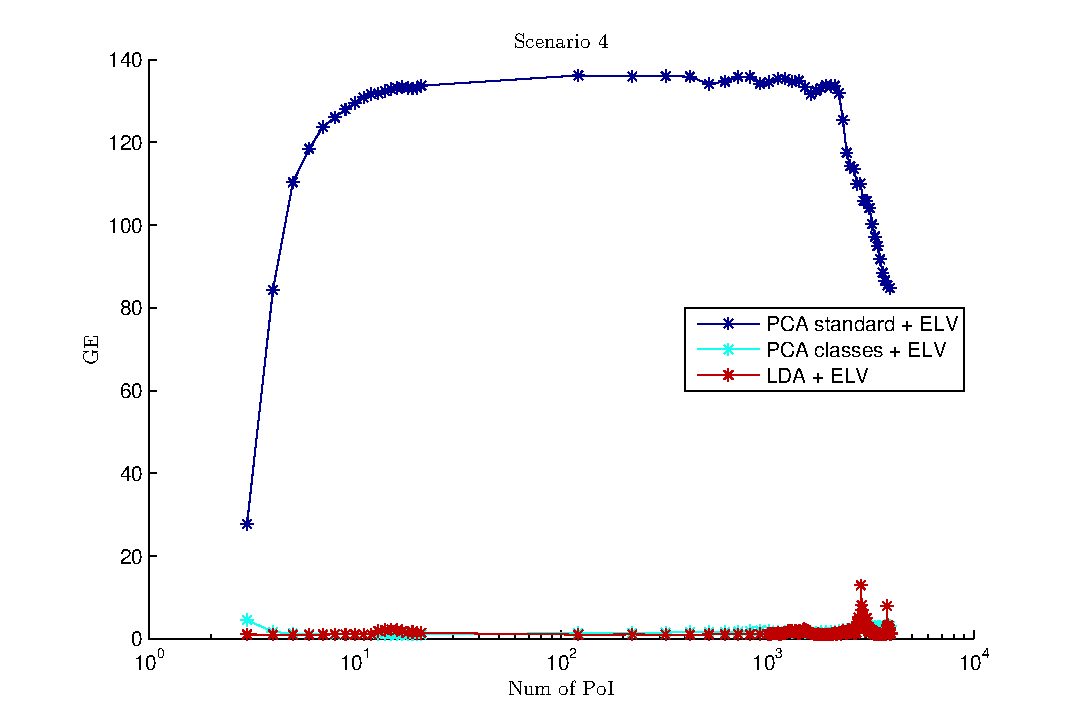
\includegraphics[width=0.5\textwidth]{figures/Criterion4.pdf}
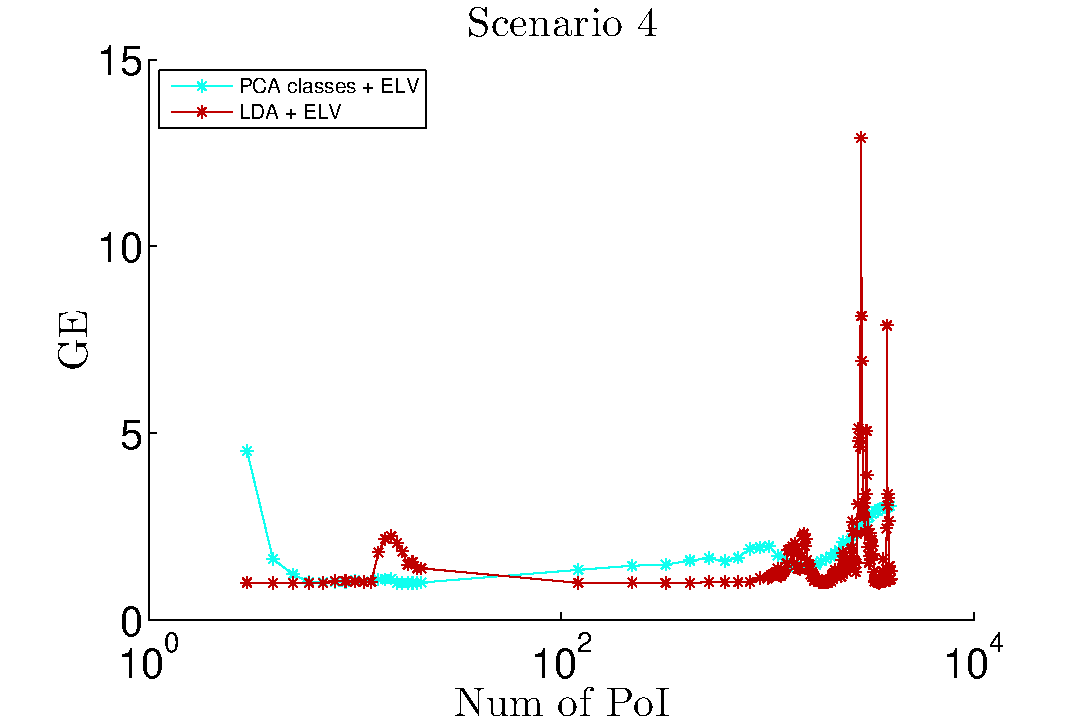
\includegraphics[width=0.5\textwidth]{figures/Criterion4cutted.pdf} 
\caption{Guessing Entropy as function of the number of original time samples the dimensionality reduction depends on.}\label{fig:4}
\end{figure}

This is the only scenario in which we allow the ELV selection method not only select the components to keep but also select interesting points within the components. To attend the wished $\numPoI$, we select couples \textit{(component, time samples)} in order of decreasing ELV, allowing the presence of only $\newTraceLength = 3$ components and $\numPoI$ globally considered.
%to make it clearer, we impose that the matrix containing the selected components as columns has exactly $\numPoI$ rows different from the zero vector. 
Looking at Fig.\ref{fig:4} we might observe that the LDA allows to achieve the maximal guessing entropy with only 1 PoI in each of the 3 selected components. 
Actually, adding PoIs worsen its performances, which is coherent with the assumption that the vulnerable information leaks in only a few points, that are excellently detected by the LDA, and that adding contribution from other points raises the noise which is then compensated by the contributions of other noisy points, in a very delicate balance. Such a behaviour is clearly visible in standard PCA case: the first 10 points considered raise the level of noise, that is then balanced by the last 1000 points.



